\section{Introduction}

For large-scale online services, such as Google, Facebook, and
Baidu, an important inter-datacenter (inter-DC) communication pattern is
{\em inter-DC bulk-data multicast}--replicating massive amounts of data
(e.g., user logs, search engine indexes, offline file sharing,
forum posts, and databases)
from one DC to many geo-distributed DCs.
%A common inter-DC communication pattern {\em bulk-data inter-DC multicast},
%which replicates data (e.g., user
%logs, search engine indexes, offline file sharing, forum posts, and
%databases) from one DC to any set of destination DCs.
Our study on the workload of
\company's\myfootnote{A large search engine provider, anonymized for
double-blind review.} DCs reveals that
inter-DC multicast amounts to 91\% of inter-DC traffic
(\Section\ref{sec:motivation}), which corroborates the findings of
other large-scale online service providers~\cite{kumar2015bwe,zhang2016piebridge}.
As data sizes continue to explode and more DCs are deployed
globally, inter-DC data transfer is expected
to grow significantly, which is a key driving force behind
recent efforts towards improving inter-DC Wide Area Network (WAN)
performance~\cite{savage1999Theend,jain2013b4,kumar2015bwe,hong2013achieving,zhang2015guarantee}.


%Global-scale online services, such as Google, Facebook, and Baidu,
%depend crucially on the ability to distribute data across
%geo-distributed datacenters (DCs) in a timely and cost-effective
%manner. This has introduced substantial challenges, as data sizes
%continue to explode and more DCs are deployed to reach a global
%footprint.
%These trends have been a key driving force behind recent efforts
%to optimize the WAN performance between two
%DCs~\cite{b4,bwe,swan,??,??,??}.


\begin{figure}[t!]
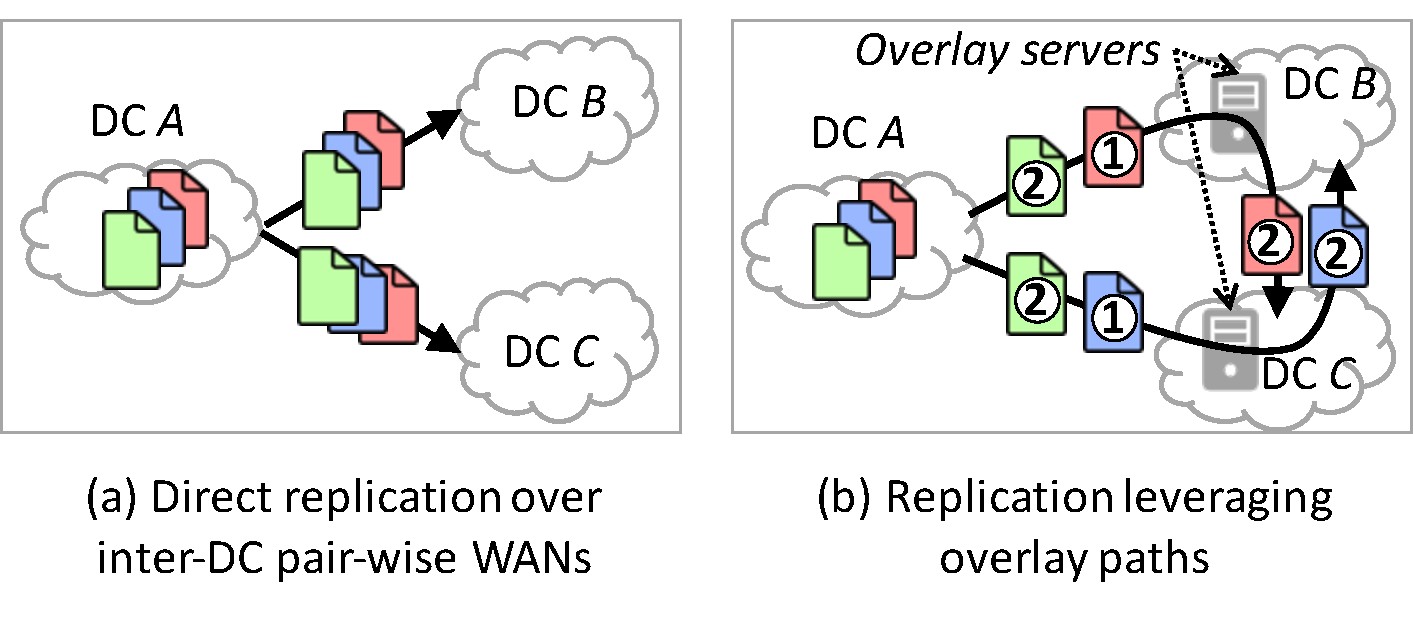
\includegraphics[width=83mm]{images/intro-example.pdf}
\vspace{-0.4cm}
\tightcaption{A simple network topology illustrating how
overlay paths reduce inter-DC multicast completion time.
%Assume the bottleneck is the outgoing router of DC $A$.
Assume each DC has 1GB/s one-directional WAN links to any other
DC, and $A$ sends 3GB data to $B$ and $C$.
Sending data from $A$ to $B$ and $C$ separately
takes 3 seconds (a),
but using overlay paths $A$$\rightarrow$$B$$\rightarrow$$C$
and $A\rightarrow$$C$$\rightarrow$$B$
simultaneously takes only 2 seconds.
The circled numbers show the order for each data piece
 is sent. }
\label{fig:intro}
\vspace{-0.4cm}
\end{figure}

Prior efforts to optimize inter-DC data replication have focused on improving the wide area network (WAN) performance
between a pair of DCs. These WAN-centric approaches, however, are insufficient as they fail to leverage
the application-level overlay paths available in
geo-distributed DCs or harness server's capability to
store-and-forward data.
As illustrated in Figure~\ref{fig:intro}, the performance of
inter-DC multicast could be substantially improved by
delivering data in parallel via multiple overlay servers
acting as intermediate points to circumvent slow WAN paths and
performance bottlenecks in DC networks.
%(More examples can be found in \Section\ref{sec:motivation}.)
Note that these overlay paths must be {\em bottleneck-disjoint} (i.e., they do
not share common bottleneck links), and
such overlay paths are available in abundance in
geo-distributed DCs (e.g., $A$$\rightarrow$$B$$\rightarrow$$C$,
$A$$\rightarrow$$C$$\rightarrow$$B$ in Figure~\ref{fig:intro}).




This paper presents {\em \name}, an {\em application-level
multicast overlay network}, which splits data into fine-grained
units and sends them in parallel via bottleneck-disjoint
overlay paths. These paths are selected dynamically in response to changes in
network conditions and the up-to-date data delivery status on each server.
%sends them in parallel on selectively picked
%overlay paths, and dynamically adapts the overlay routes and
%schedules in response to changes in network conditions and
%workload churns.
Note that \name selects application-level overlay paths and is
complementary to network-layer techniques that
improve the WAN performance.
While application-level multicast overlays have been applied
in other contexts
(e.g.,~\cite{Liebeherr2002Application,Wang2007mTreebone,
Andreev2013Designing,Mokhtarian2015Minimum}), building one
for large online service providers poses two
challenges.
%Building on the operational experience of
%\company\footnote{Anonymized for double-blind reviewing},
%a large online service providers, we summarize two challenges,
%which to our best knowledge do not have direct solution.
First, as each DC has tens of thousands of servers, the
resulting sheer amounts of overlay paths make it
unwieldy to update overlay routing decisions in real time.
The performance could be suboptimal by simply borrowing techniques
from prior work, such as servers making local reactive
decisions~\cite{kostic2003bullet,Repantis2010Scaling,Huang2014A},
or pruning the set of overlay paths by strictly
structured (e.g., layered) topologies~\cite{Nygren2010The}.
Second, a small increase in the delay of latency-sensitive traffic
can cause significant revenue loss, so the bandwidth usage
of inter-DC bulk-data multicasts must be tightly controlled
to avoid interference with latency-sensitive
traffic\myfootnote{Despite priority-based queuing
at each DC border router, bulk-data multicasts compete
inter-DC WAN (not managed by \company) with
latency-sensitive traffic, leading to negative impacts on
latency-sensitive traffic.}.
%, even at the expense of a slightly lower link utilization.

%Inspired by the multicast overlay networks, we argue that to optimize bulk-data multicast,
%a similar {\em application-level multicast
%overlay network} is needed to optimally deliver data in a way that
%fully utilizes inter-DC overlay paths.
%To replicate a data file from one DC to multiple DCs, this overlay
%multicast network will send different parts of the data
%simultaneously along selectively picked overlay paths, and
%dynamically adapt the overlay routing in response to changes in
%network conditions and resource availability.




%we argue that an {\em inter-DC multicast
%overlay} network that optimally schedules and routes data via
%overlay paths is essential to ensuring the desirable performance
%for two reasons.
%First, the need for multicasting data to a subset of (or all) DCs
%is endemic in online service providers; e.g.,
%Google has seen a \fillme-fold increase in \fillme years
%in the amount of data that needs to be distributed to all
%DCs~\cite{??}, and this number would only multiply with more
%DCs deployed.
%Second, the improved WAN performance between any DC pair can be
%fully utilized only when used with an inter-DC multicast overlay
%network that
%splits data in fine granularities and optimally select
%overlay paths to circumvent inter-/intra-DC bottlenecks.



%%While these efforts have shown promising improvement on the performance of pairwise
%%inter-DC WANs, we argue that an efficient multicast overlay network that optimally
%%schedules and routes data from each DC to multiple DCs via inter-DC overlay paths
%%is essential to ensuring desirable performance and fully utilizing the improved
%%pairwise inter-DC data transfer.
%While multicast overlay networks have been studied extensively
%in settings of peer-to-peer (P2P) streaming~\cite{??,??} and
%content delivery networks (CDNs)~\cite{??,??}, it remains unclear
%whether existing approaches apply to the scale of large online
%service providers like Google and Baidu.
%%The conventional wisdom has been that to operate at scale and react
%%in real time, one has to either organize overlay nodes in a
%%strictly structured (and thus suboptimal) topology
%%(e.g.,~\cite{akamai}), or use a hybrid (and thus more
%%complex) control mechanism (e.g.,~\cite{vdn}) with a local
%%logic adapting in real time and a global logic updating every
%%few minutes.
%Drawing on the operational experience from
%\company\footnote{Anonymized for double-blind reviewing}, a large
%online service providers, we see two key requirements
%of an inter-DC multicast overlay network.
%First, because these DCs have more servers and thus
%exponentially more overlay paths than CDNs or P2Ps,
%it is untenable to exploit all overlay paths by
%traditional approaches, such as decentralized or hybrid path
%selection (e.g.,~\cite{??,??}), or structured topologies
%(e.g.,~\cite{akamai}).
%Second, these WANs are shared by latency-sensitive traffic
%and bulk background traffic.
%Because any small increase in delay of
%latency-sensitive traffic can cause substantial revenue losses,
%there is a strong need to prevent interference on
%latency-sensitive traffic, even at the expense of slightly lower
%link utilization.


%while a more decentralized overlay network protocol
%is conceptually simpler, it is untenable for them to fully
%utilize the overlay paths, so we see a great room for
%improvement, especially at tail performance. This motivates
%the fully centralized architecture that maintains a fresh
%global view for decision making.
%Second, adding even a small delay in latency-sensitive data
%can cause significant revenue losses. Therefore, it is
%acceptable to enforce a clean bandwidth separation between
%bulk traffic delivery and latency-sensitive data, even at
%the cost of lower link utilization.
%
%But designing a multicast overlay for DCs of online service
%providers is different in two key aspects.
%First, these DCs have more servers in DCs, and much more overlay
%paths, so it is necessary to maintain an up-to-date global view
%of data delivery status on all servers to fully exploit these
%paths.
%Second, the WANs are shared by latency-sensitive user data and
%background bulk data, creating a need for minimizing the data
%distribution latency while preventing negative
%impacts on the latency-sensitive data.

To address these challenges, \name fully {\em centralizes}
the scheduling and routing of inter-DC multicast.
Contrary to the intuition that servers must retain certain
local decision-making capability to achieve scalability and
responsiveness, \name's centralized design
is built on two observations (\Section\ref{sec:overview}):
(1) While it is less likely to make
centralized decisions in real time, most multicast data transfers
last for tens of seconds and thus can tolerate certain delay incurred by
the central controller in order to make optimal control based on a global view.
(b) Centrally coordinated bandwidth allocation is amenable
to minimizing interference between inter-DC multicast
traffic and latency-sensitive traffic.% by enforcing bandwidth allocation on overlay paths.
%(c) Finally, a centralized design is amenable to a simple
%implementation from an engineering perspective;
%e.g., the program running locally on the server side is
%only triggered by data arrivals or control messages, and
%thus can be largely stateless.

%This paper presents {\em \name}, a near-optimal multicast
%overlay network for inter-DC bulk data multicast.
%At the core of \name is the decision of {\em fully centralizing
%the scheduling and routing of bulk-data multicast}.
%%This paper presents {\em \name}, a near-optimal inter-DC multicast
%%overlay network, which minimizes data distribution delay from one
%%DC to any subset DCs by dynamically splitting,
%%reordering, and deliver data via overlay paths selected
%%from all server-level paths between the source DC and destination DCs.
%%\name focuses on distributing background bulk data (e.g., \fillme),
%%which is by several orders of magnitudes larger than
%%latency-sensitive user data.
%Contrary to the intuition that, in order to scale out
%and be responsive, servers must retain the capability to make
%certain local decisions, \name's centralized design
%is built on the several empirical observations:
%\begin{packeditemize}
%\item First, while it is indeed impractical to update centralized
%decision-making in real-time, bulk-data transfers, which take
%at least tens of seconds, can tolerate a small update delay in
%overlay routing decisions
%in the hope of getting closer-to-optimal decisions based on
%a global view of data delivery status.
%\item Second, centrally coordinated decision-making makes it easier
%to enforce bandwidth allocation on all overlay paths,
%and thus eliminate interference of bulk-data
%transfers on latency-sensitive traffic.
%\item Finally, a centralized design is amenable to a simple
%implementation from an engineering perspective;
%e.g., the program running locally on the server side is
%only triggered by data arrivals or control messages, and
%thus can be largely stateless.
%\end{packeditemize}


The key to realizing \name's benefits in practice is to update
the overlay network on the timescale of seconds in response to dynamic network conditions
and failures. \name achieves this by {\em decoupling} its centralized control
into scheduling of data transfers and
overlay routing of individual data transfers.
This decoupling attains provable optimality and at the same time
allows \name to update overlay network routing and scheduling in
a fraction of second (4 orders of magnitude faster than without decoupling
routing and scheduling) on production workloads
of a large online service provider (e.g., sending $10^5$s of data blocks
simultaneously along $10^4$s of disjoint overlay paths, and updating
the routing every other second).


%At the core of \name are two design choices.
%\begin{packeditemize}
%\item {\em Centralized decision-making:}
%Decision making in \name is fully centralized; the \name
%controller maintains a global view of data delivery status on
%all servers
%and makes overlay routing and scheduling decisions every
%few seconds (by default, 3 seconds).
%\name solves a multicommodity problem using
%a near-optimal algorithm amenable to efficient incremental
%updates.
%\item {\em Clean bandwidth separation:}
%To prevent delay caused by background data on
%latency-sensitive user data, \name monitors the
%aggregated traffic volume
%of latency-sensitive data, and maintains a clean, dynamic
%bandwidth
%separation by enforcing the maximum amount of bulk-data
%multicast sent from each server.
%\end{packeditemize}

%While \name's design choices introduce performance costs (i.e.,
%\name does not update decisions in real time or achieve full
%link utilization), our design philosophy is that these costs are
%favorably outweighed by several benefits.
%% of near-optimal global optimization
%%as well as the resulting simpler solution from an engineering
%%perspective.
%%This observation inspired the key insight underlying \name that
%%multicasting bulk data can tolerate a small amount of delay in
%%exchange for closer-to-optimal decisions overlay routing and
%%scheduling.
%(1) Since delivering bulk data takes tens of seconds to
%minutes, \name can tolerate a delay of updating centralized
%control decisions at coarse timescales of several
%seconds in exchange for closer-to-optimal decisions made by
%the centralized controller.
%(2) The observation that the aggregation of
%latency-sensitive traffic tends to
%be stable on timescales of several seconds suggests that it is
%plausible to eliminate undesired interference on
%latency-sensitive traffic by clean bandwidth separation
%while achieving a high link utilization.
%%Moreover, having a global view on the delivery status of all objects in all
%%servers allows the controller to remarkably improve overlay routing and
%%scheduling decisions, which would be impossible otherwise.
%(3) Finally, these design choices are amenable to a simple
%implementation from an engineering perspective;
%e.g., the program running locally on the server side is
%only triggered by data arrivals or control messages, and
%thus can be largely stateless.


We have implemented a prototype of \name and integrated it in
\company, one of the largest search service providers.
We deployed \name in 10 DCs and ran a pilot study on 500 TB
data for over 7 days.
Our real-world experiments show that \name achieves 3-5$\times$
speedup over \company's existing solution, and it can reduce
incidents of excessive bandwidth consumption by bulk-data
transfers.
Using real trace-driven evaluation and microbanchmarking,
we also show that \name outperforms techniques widely used in
CDNs, can handle the workload of \company's
inter-DC multicast traffic with one general-purpose server,
and can tolerate various failure scenarios.


Our contributions are summarized as following:
\begin{packeditemize}
\item Characterizing the workload of inter-DC bulk-data
replication to motivate the need of application-level
multicast overlay networks (\Section\ref{sec:motivation}).
\item Designing \name, an application-level
multicast overlay network which achieves near-optimal flow completion
time with a centralized control scheme (\Section\ref{sec:overview},\ref{sec:logic},\ref{sec:system}).
\item Demonstrating the practical benefits of \name by a real-world
 deployment in a large online service provider (\Section\ref{sec:evaluation}).
\end{packeditemize}
